\chapter[Área acessível M]{Área Acessível (M), BAM Framework e Seleção de Background}

\begin{objetivos}
	Ao final desta unidade, o estudante deverá compreender o conceito de área acessível (M); interpretar o framework BAM; diferenciar área de estudo, área de calibração e área de projeção; delimitar uma área M biologicamente defensável; gerar pontos de background; comparar background no bioma inteiro versus background restrito à área M; e preparar dados de presença-background para modelagem de \textit{Dinizia excelsa}.
\end{objetivos}

\section{Introdução}

A definição da área acessível, frequentemente representada pela letra \(M\), é uma das decisões mais importantes em Modelagem de Distribuição de Espécies. A área \(M\) representa a porção do espaço geográfico que esteve historicamente acessível à espécie por dispersão, história biogeográfica, conectividade e ausência de barreiras intransponíveis \parencite{soberon2005,soberon2007,soberon2009,barve2011crucial}.

Em SDM, a área \(M\) influencia diretamente a seleção de background, a disponibilidade ambiental, os contrastes entre presença e ausência/background e, consequentemente, os parâmetros estimados pelos modelos. Uma área \(M\) muito ampla pode incluir ambientes nunca acessíveis à espécie; uma área muito restrita pode excluir gradientes relevantes para estimar seu nicho.

\begin{conceito}[title={\faBook\quad Área acessível (M)}]
	A área acessível (M) é o conjunto de regiões que a espécie poderia ter alcançado ao longo de sua história recente, considerando dispersão, barreiras, conectividade da paisagem e história biogeográfica. Ela não é necessariamente igual ao bioma inteiro nem à distribuição observada da espécie.
\end{conceito}

\section{BAM framework}

O framework BAM organiza a distribuição das espécies como resultado da interação entre três componentes principais: fatores bióticos (B), fatores abióticos (A) e área acessível por dispersão (M). Em termos simplificados, uma espécie ocorre onde as condições ambientais são adequadas, as interações bióticas permitem sua persistência e a região é acessível historicamente.

\begin{equationbox}
	\[
	G_O = A \cap B \cap M
	\]
	
	em que \(G_O\) representa a distribuição observada; \(A\), as condições abióticas adequadas; \(B\), as interações bióticas permissivas; e \(M\), a área acessível.
\end{equationbox}

\begin{atencao}[title={\faExclamationTriangle\quad Área M não é detalhe técnico}]
	A definição de \(M\) altera o conjunto de condições ambientais disponíveis para o modelo. Portanto, ela deve ser justificada biologicamente e não escolhida apenas por conveniência computacional.
\end{atencao}

\section{Delimitação da área M para \textit{Dinizia excelsa}}

Nesta unidade, a área \(M\) será delimitada de forma operacional a partir dos registros finais de \textit{Dinizia excelsa}, usando um buffer espacial ao redor das ocorrências e restringindo o resultado ao limite do bioma Amazônia. Essa abordagem é didática e reprodutível, adequada para construir a base das próximas unidades de modelagem.

\rscriptfile{scripts/unidade05/01_estrutura_pastas.R}

\rscriptfile{scripts/unidade05/02_delimitar_area_m_dinizia.R}

\begin{figure}[H]
	\centering
	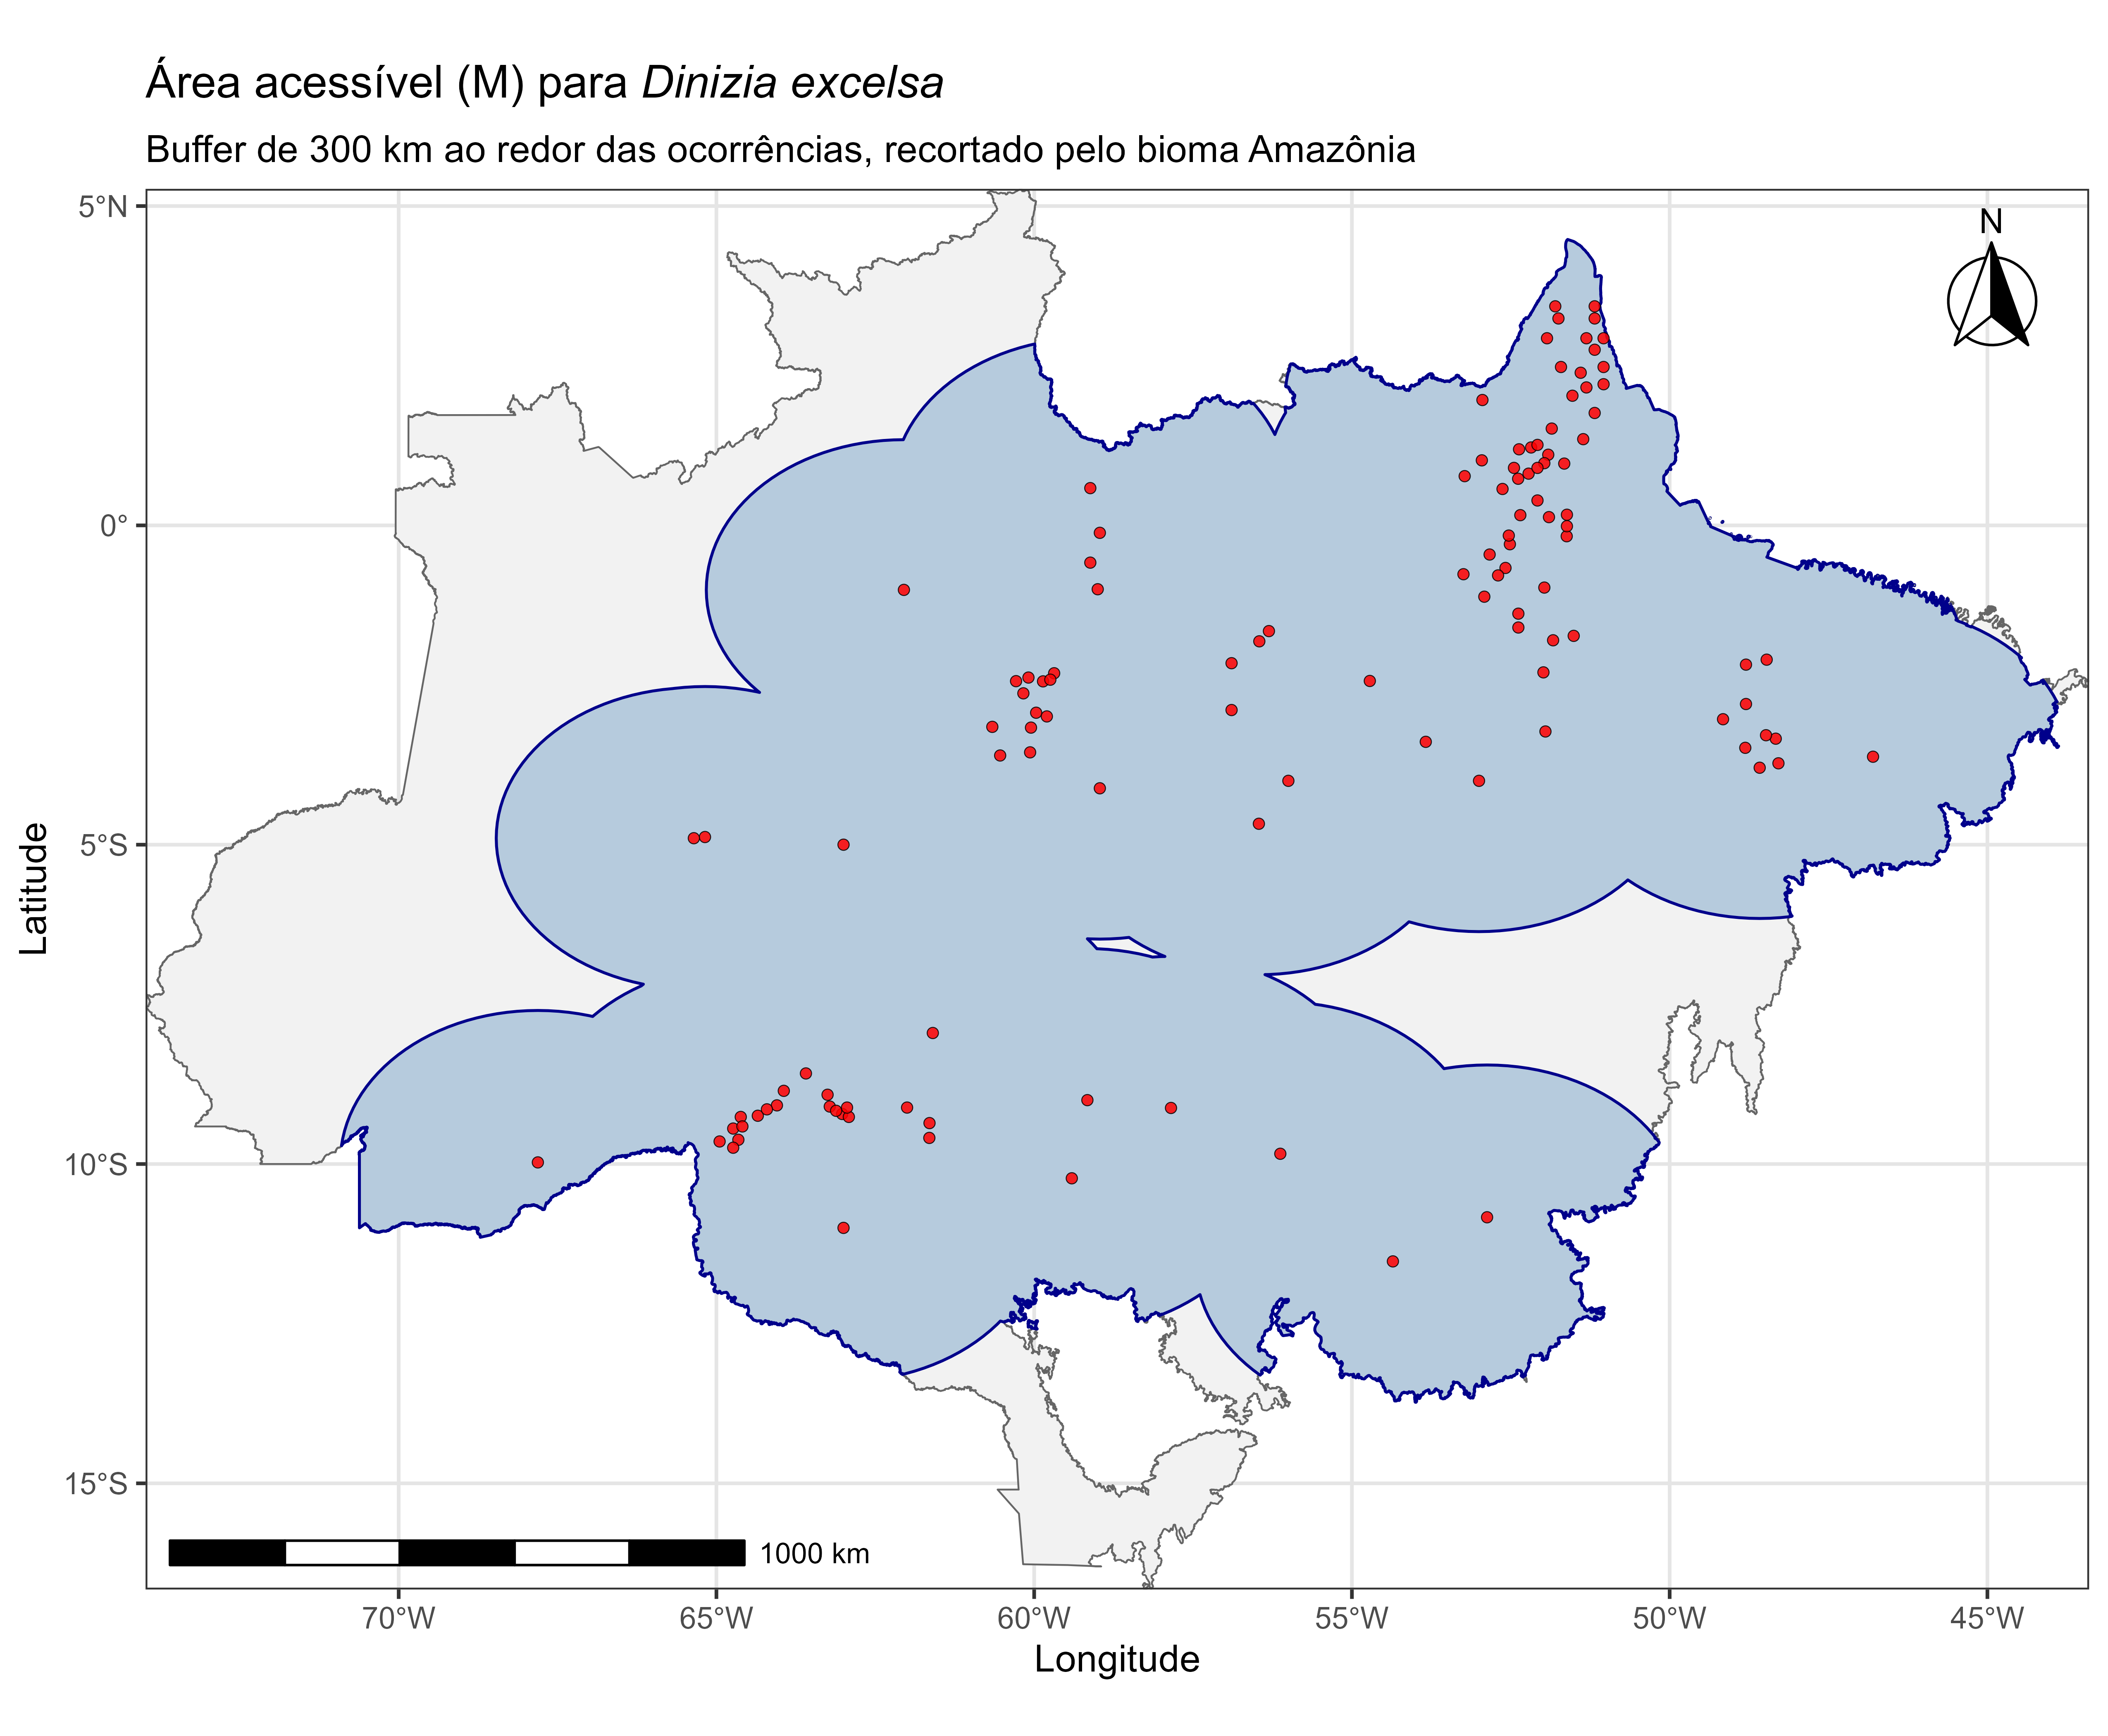
\includegraphics[width=0.90\textwidth]{figuras/unidade05/unidade05_area_m_dinizia.png}
	\caption{Área acessível (M) delimitada para \textit{Dinizia excelsa} no bioma Amazônia. A área foi definida por buffer espacial ao redor das ocorrências e recortada pelo limite do bioma.}
	\label{fig:unidade05_area_m_dinizia}
\end{figure}

\section{Seleção de background}

Pontos de background representam o ambiente disponível para calibração do modelo. Em modelos presença-background, eles não são ausências verdadeiras. Eles caracterizam as condições ambientais disponíveis dentro da área considerada acessível.

\rscriptfile{scripts/unidade05/03_gerar_background_area_m.R}

\begin{figure}[H]
	\centering
	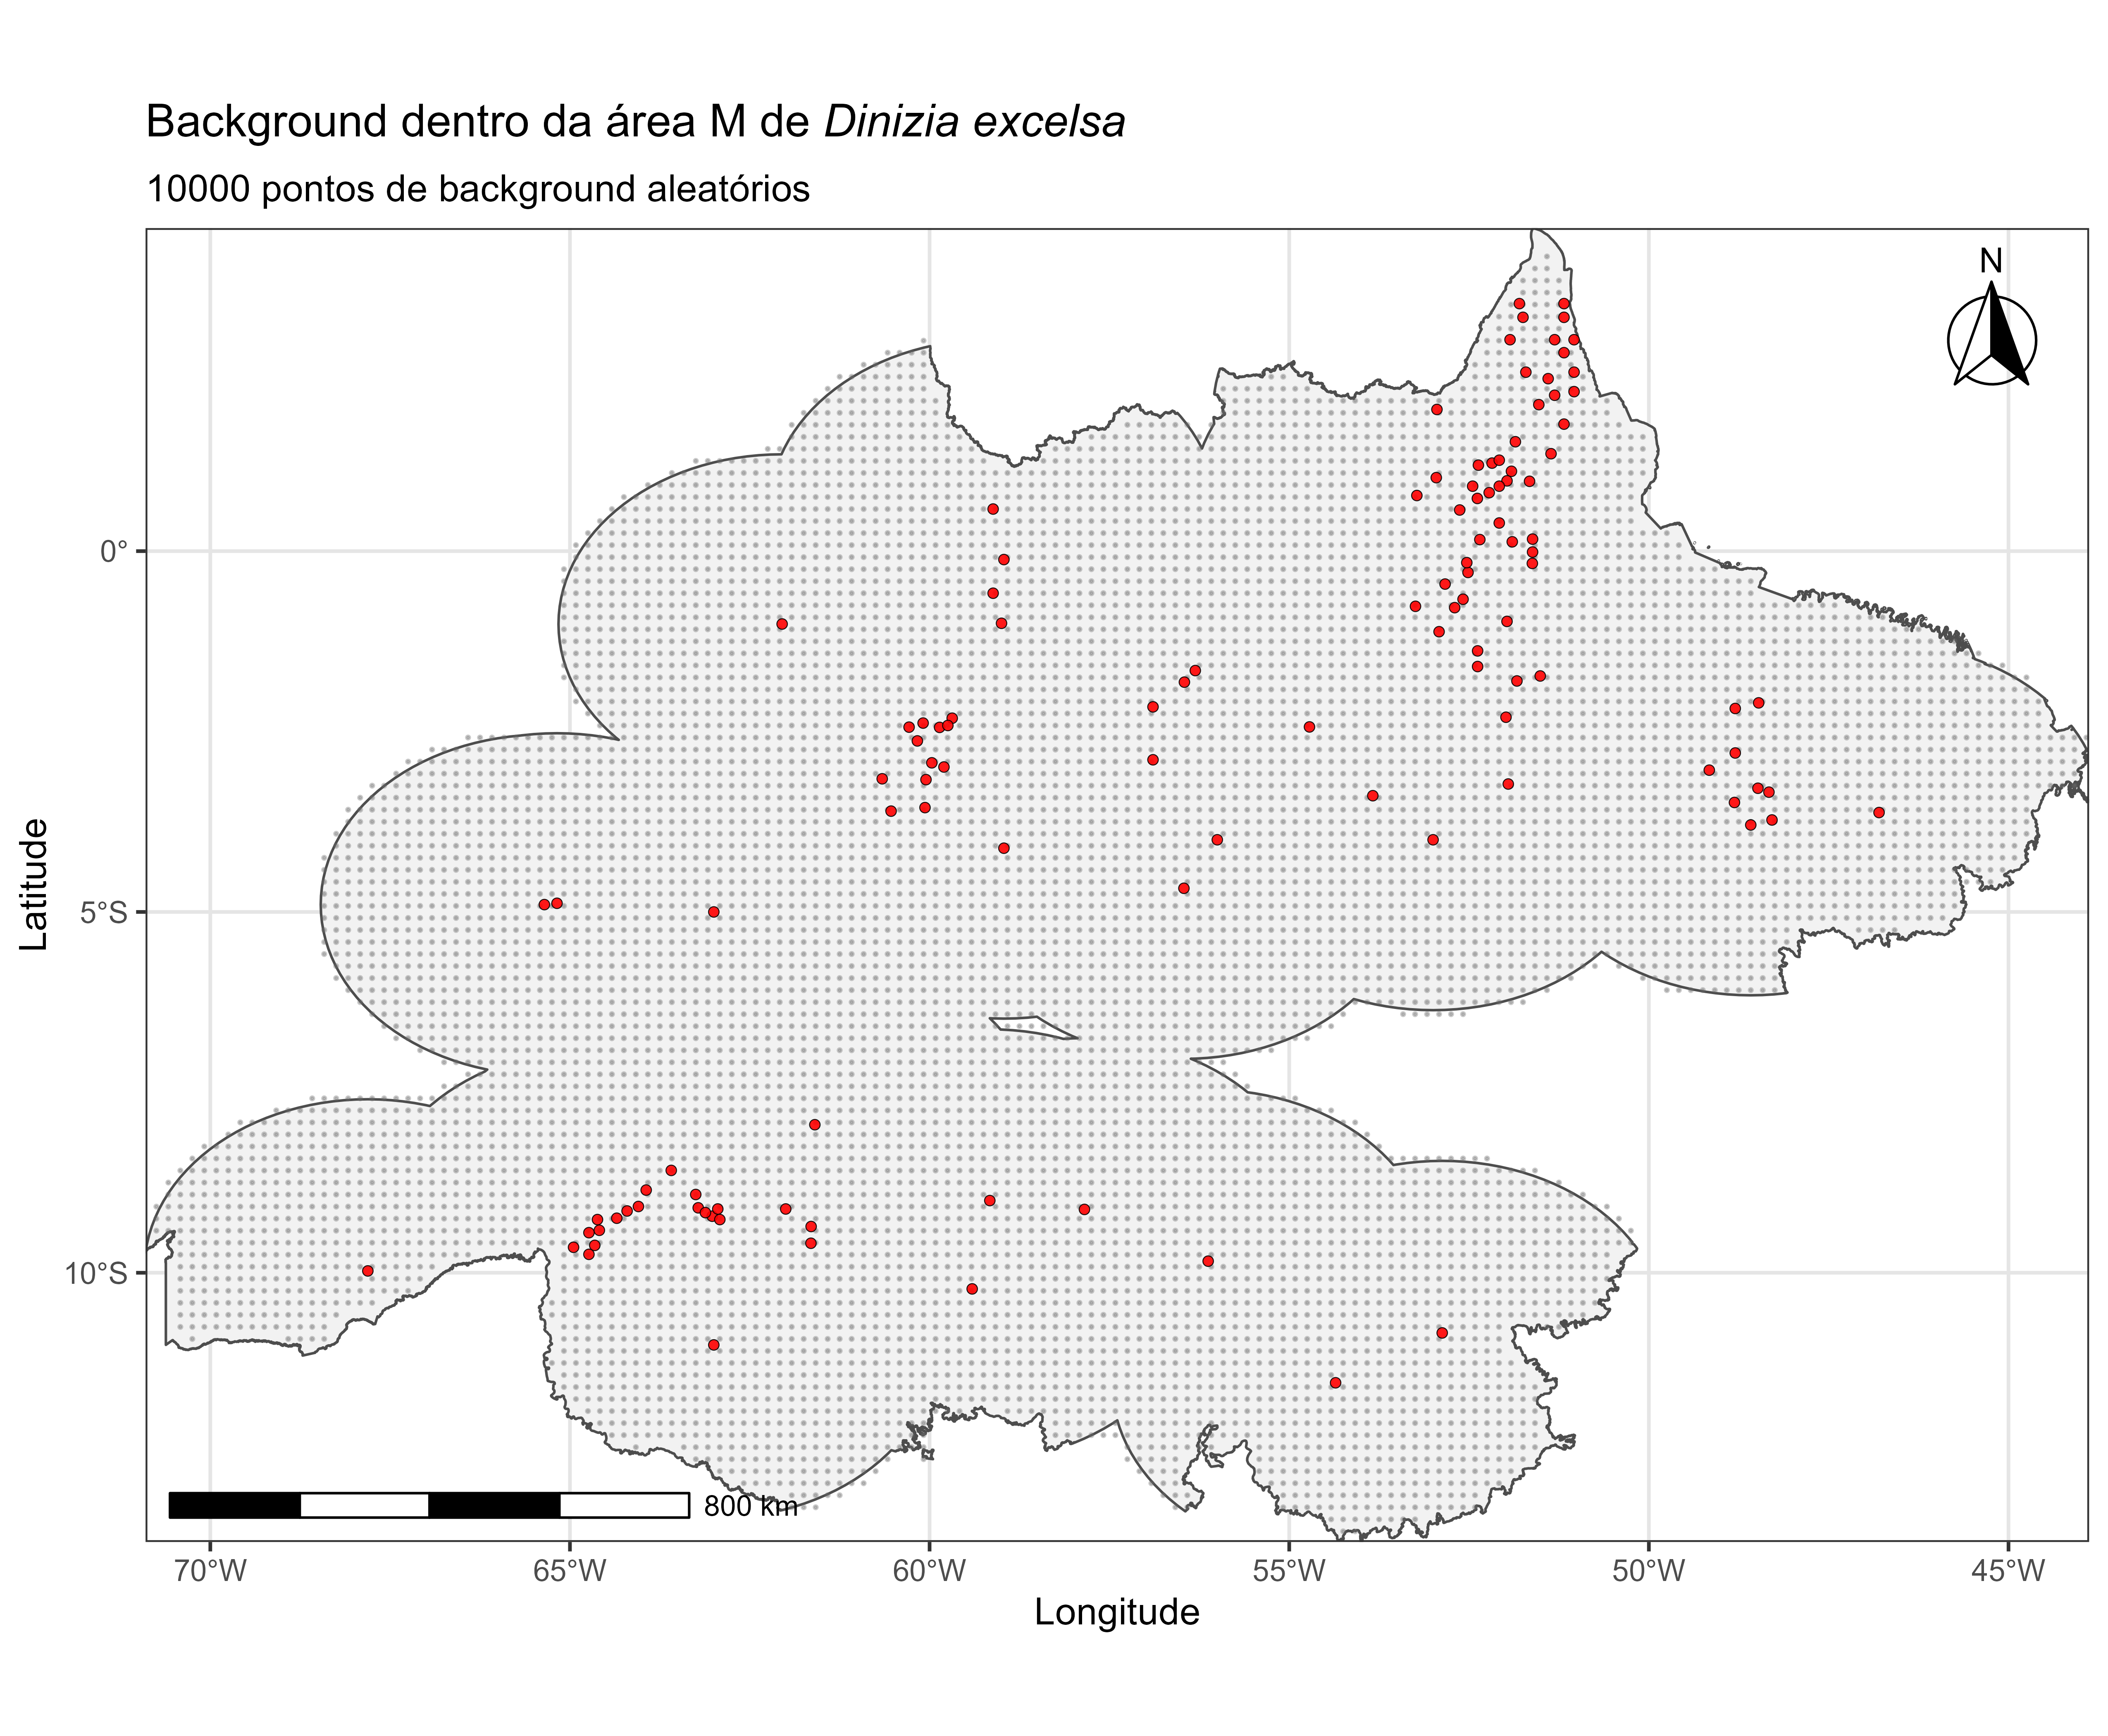
\includegraphics[width=0.90\textwidth]{figuras/unidade05/unidade05_background_area_m.png}
	\caption{Pontos de background gerados dentro da área acessível (M) para \textit{Dinizia excelsa}.}
	\label{fig:unidade05_background_m}
\end{figure}

\section{Background no bioma versus background na área M}

A seleção do background pode alterar substancialmente a distribuição ambiental disponível para o modelo. Por isso, é útil comparar o background amostrado no bioma inteiro com o background restrito à área \(M\).

\rscriptfile{scripts/unidade05/04_comparar_background_bioma_m.R}

\begin{figure}[H]
	\centering
	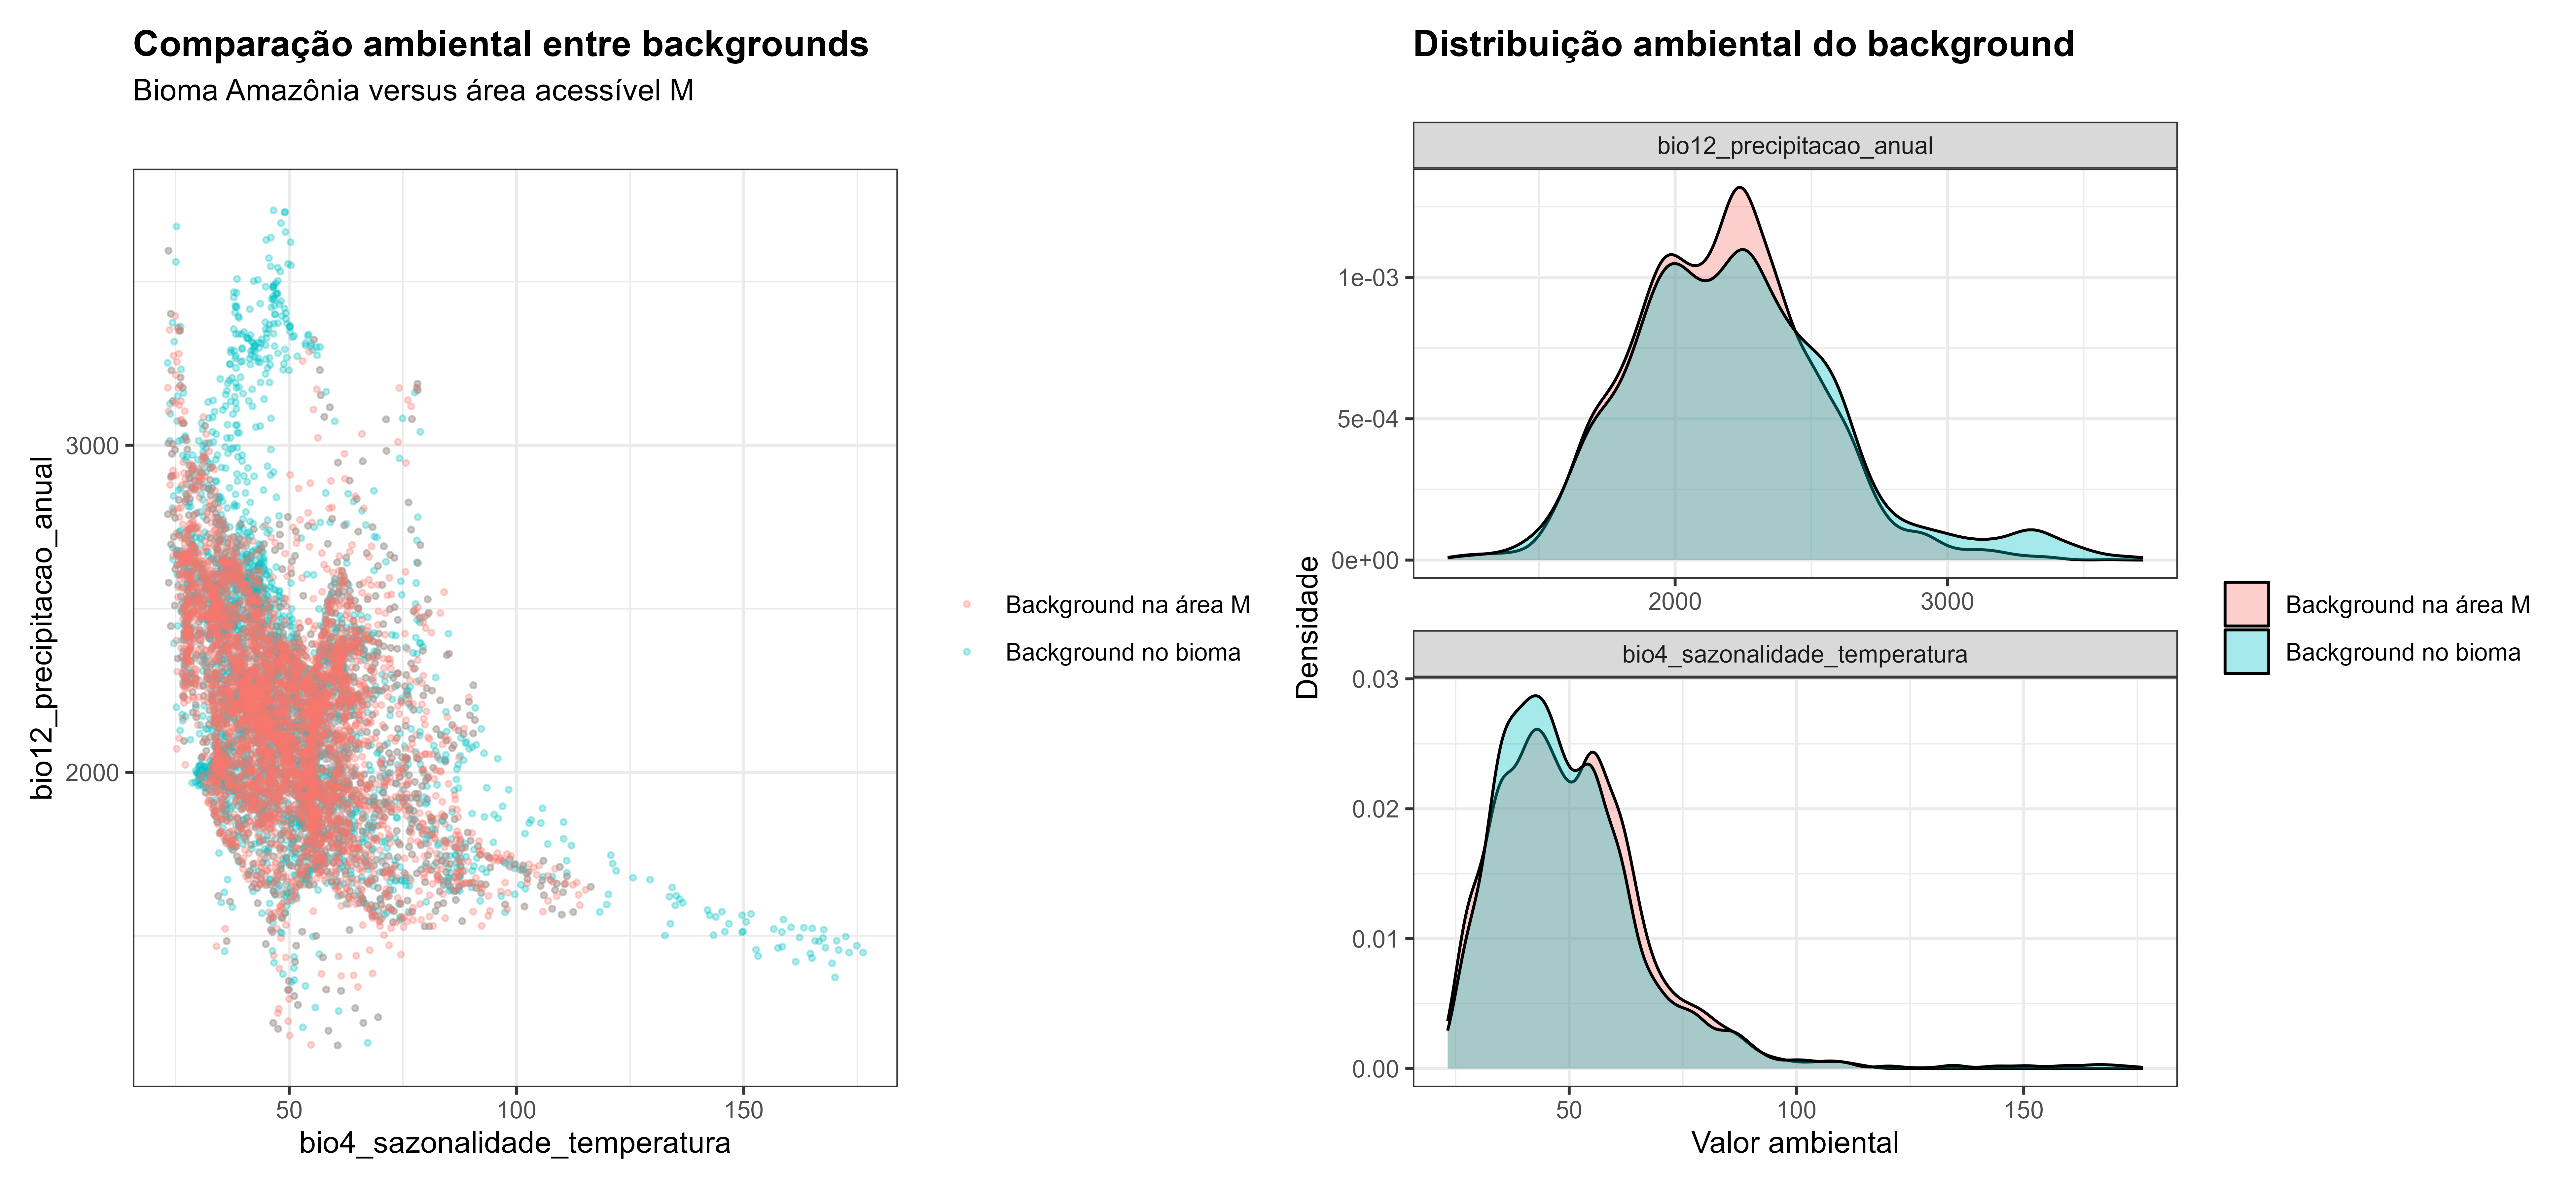
\includegraphics[width=0.90\textwidth]{figuras/unidade05/unidade05_comparacao_background.png}
	\caption{Comparação entre background amostrado no bioma Amazônia e background restrito à área acessível (M).}
	\label{fig:unidade05_comparacao_background}
\end{figure}

\section{Extração ambiental e base presença-background}

A última etapa consiste em extrair os valores das variáveis ambientais selecionadas nas presenças e nos pontos de background da área \(M\), construindo a base presença-background que será usada nas unidades seguintes.

\rscriptfile{scripts/unidade05/05_preparar_presenca_background.R}

\begin{figure}[H]
	\centering
	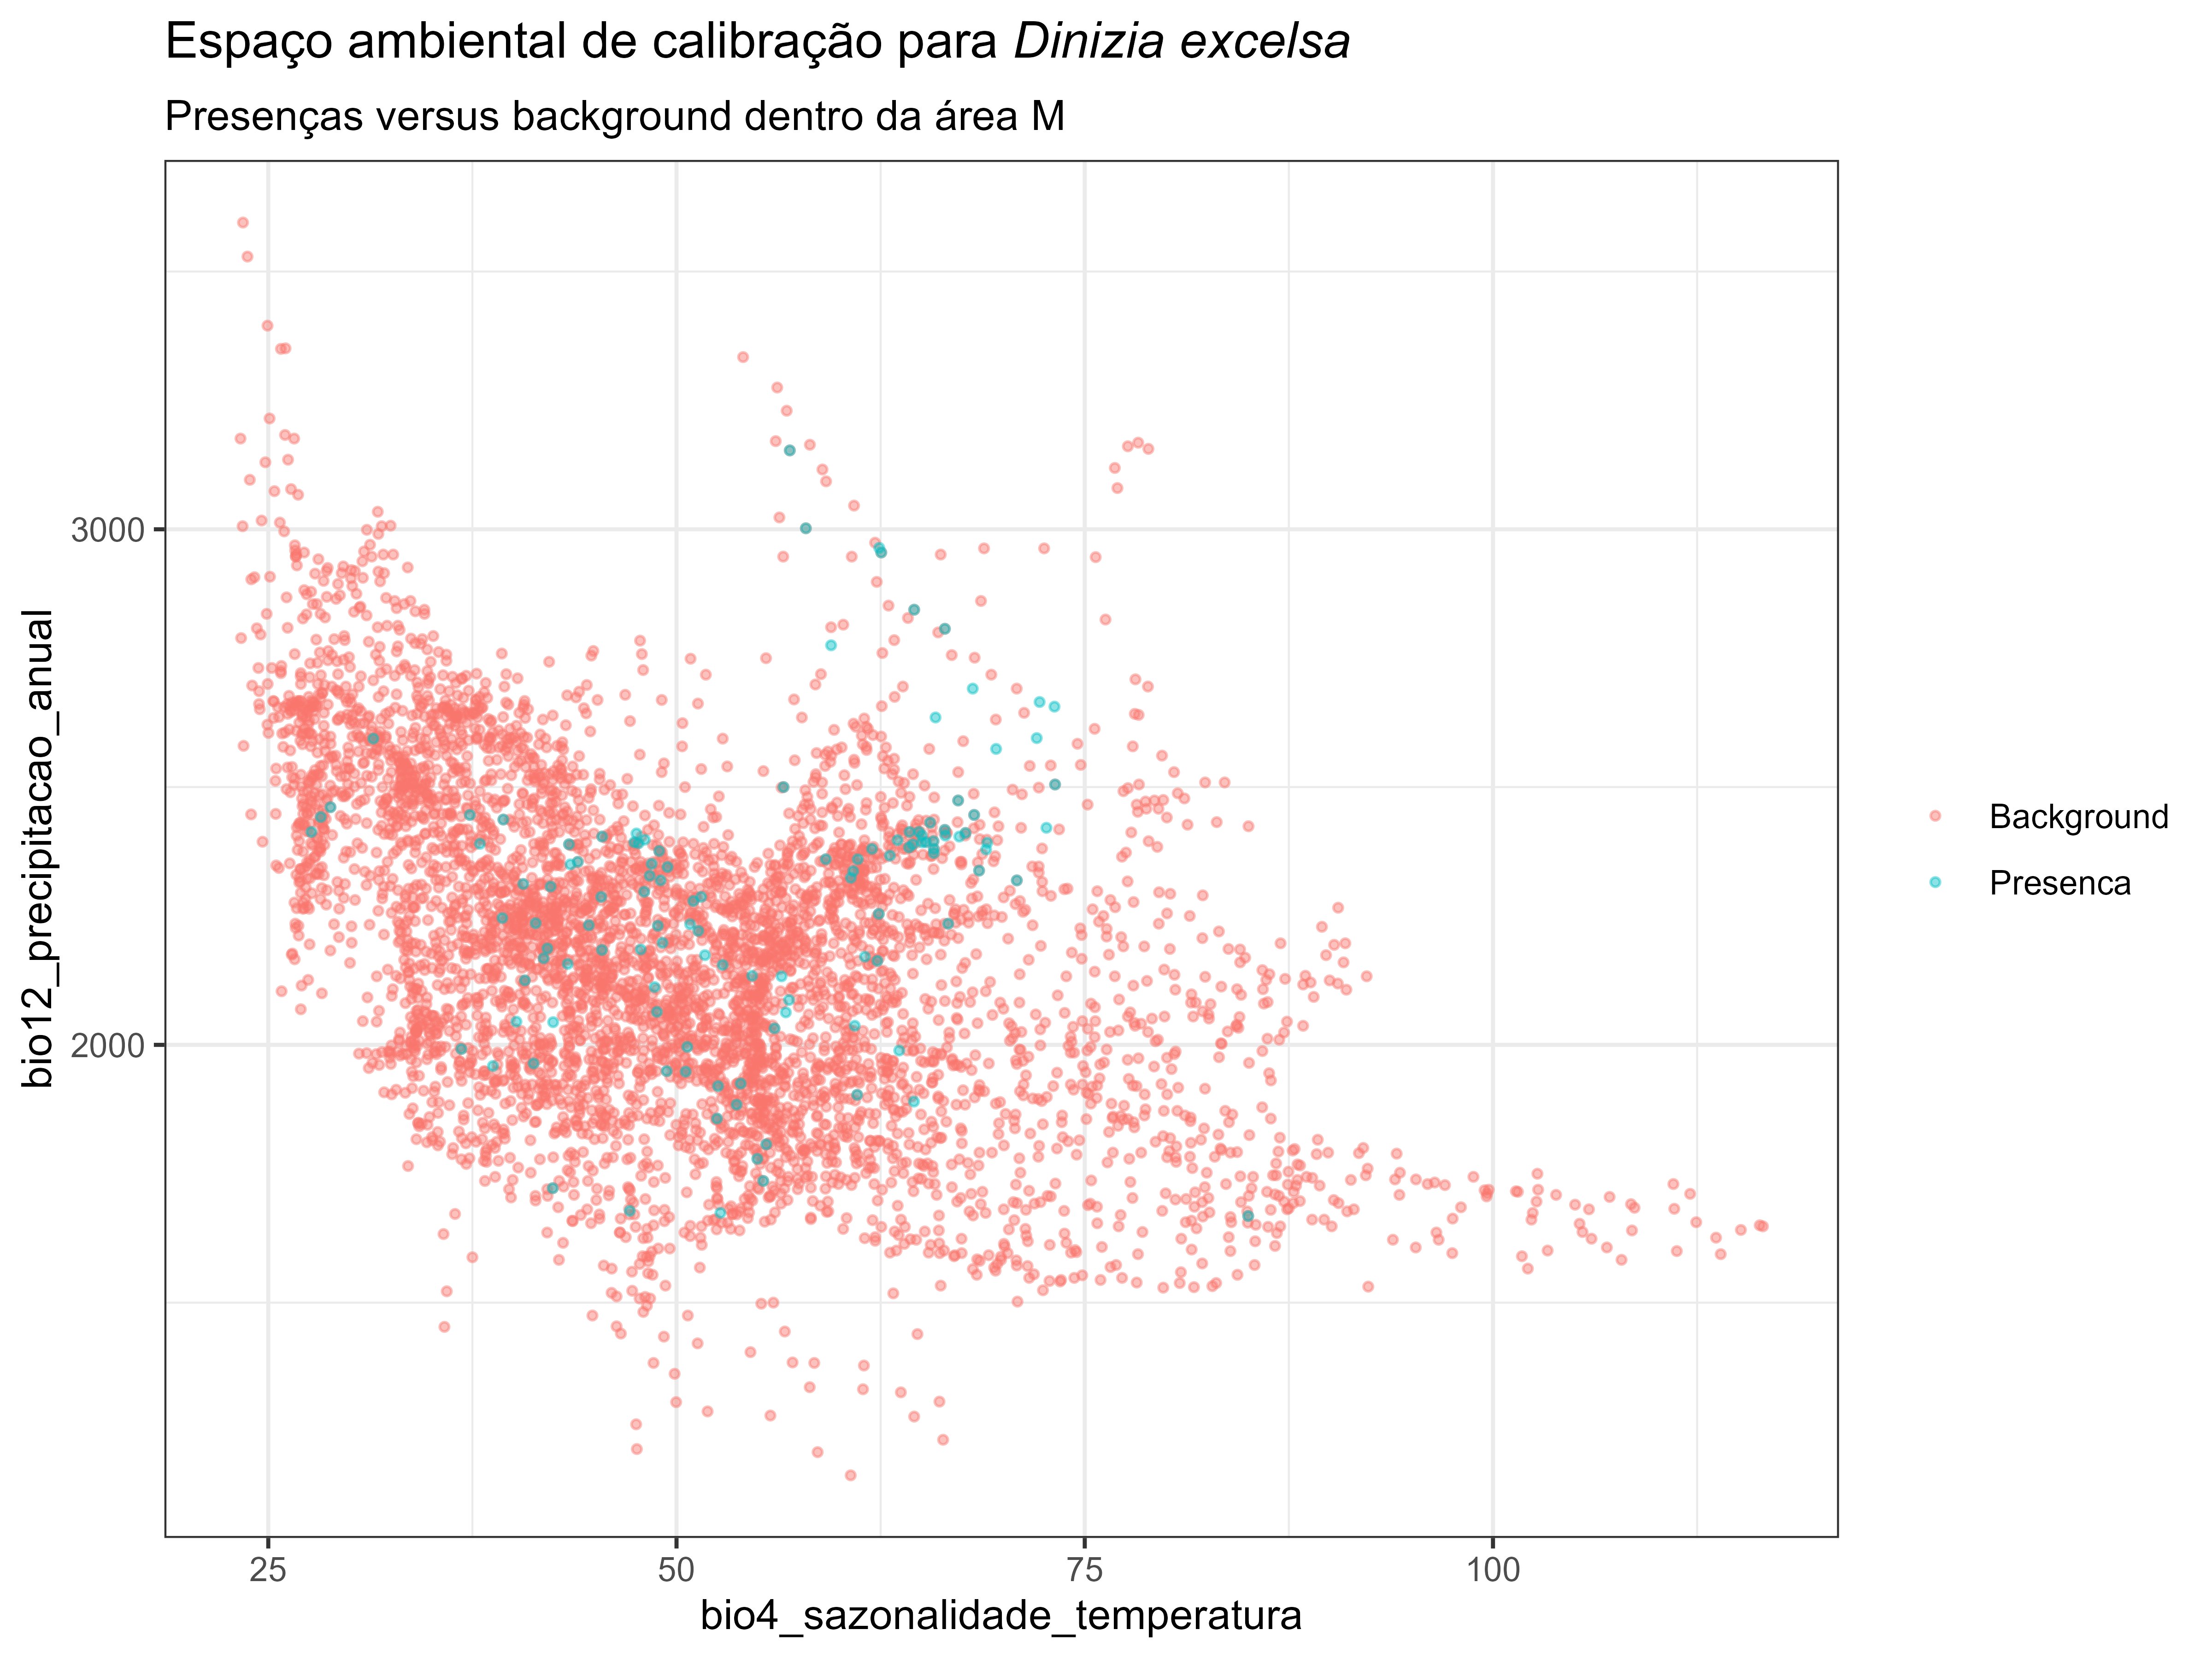
\includegraphics[width=0.86\textwidth]{figuras/unidade05/unidade05_espaco_ambiental_presenca_background.png}
	\caption{Espaço ambiental comparando presenças de \textit{Dinizia excelsa} e background dentro da área acessível (M).}
	\label{fig:unidade05_espaco_presenca_background}
\end{figure}

\section{Pipeline completo}

\rscriptfile{scripts/unidade05/06_pipeline_area_m_background.R}

\section{Síntese da unidade}

A definição da área acessível (M) é uma decisão ecológica, biogeográfica e metodológica. Ela influencia o background, a calibração, a avaliação e as projeções dos modelos. Para \textit{Dinizia excelsa}, a delimitação operacional de \(M\) no bioma Amazônia fornece uma base coerente para os modelos das próximas unidades.

\begin{conceito}[title={\faBook\quad Mensagem central}]
	Em SDM, o background deve representar o ambiente disponível para a espécie dentro da área acessível. Modelos calibrados com background inadequado podem produzir mapas biologicamente frágeis, mesmo quando apresentam boas métricas estatísticas.
\end{conceito}

% ============================================================
% UNIDADE 6
% ============================================================

